\begin{appendices}
    \renewcommand\thefigure{\thesection.\arabic{figure}}
    \appendixheaderon
    \section{Graphiques}
    \label{ann:graphiques}

    \subsection{Fonction logistique}
    \begin{figure}[ht]
        \centering
        \label{ann:cycles}
        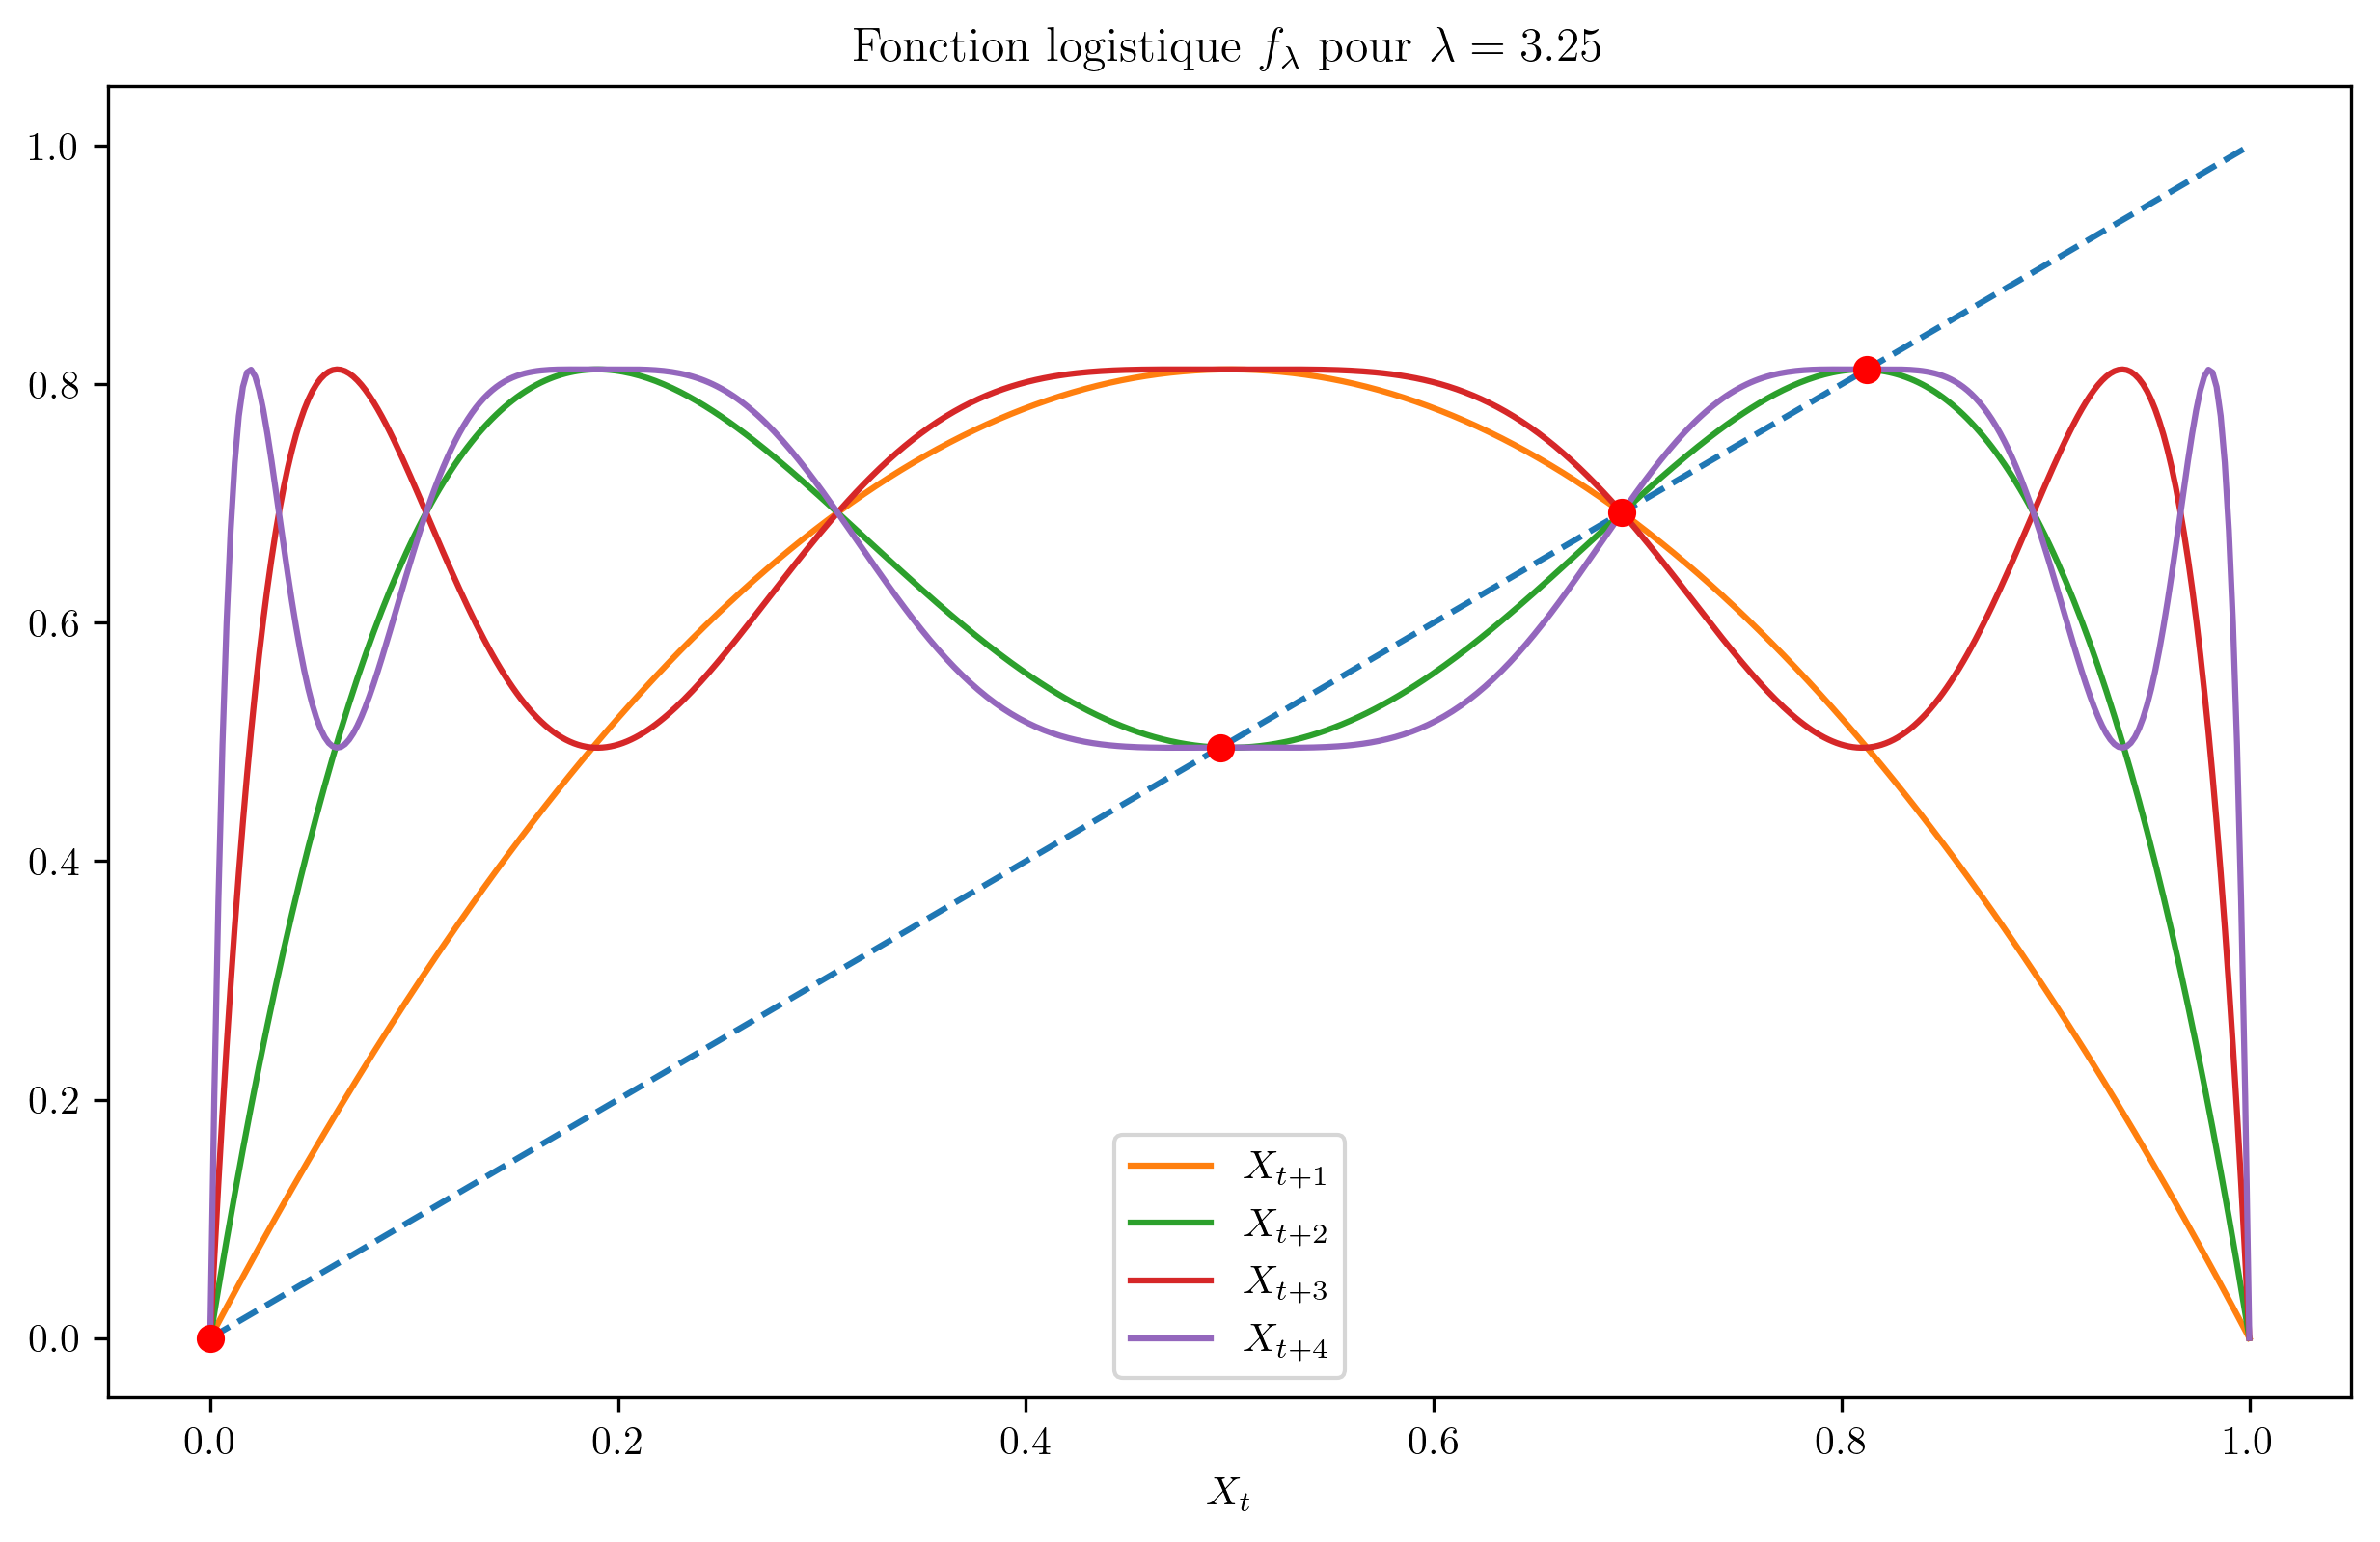
\includegraphics[width=\textwidth]{fct_log_recap.png}
        \caption{Fonction Logistique}
    \end{figure}

    \newpage
    \section{Codes python}
    \label{ann:code}

    \subsection{Génération de la fonction logistique}
    \begin{minted}{python}
# Taux d'accroissement (lambda)
a = 3.25
# Génération du vecteur des abscisses
x = np.linspace(0,1,500)
# Génération du vecteur des ordonnées
delta = x
y1 = logistical(x, a)
y2 = logistical(y1, a)
y3 = logistical(y2, a)
y4 = logistical(y3, a)

# Création de la figure (taille en pouces optionnelle)
fig = plt.figure(figsize=(10,6), dpi=300)

ax = fig.add_subplot(1,1,1)

# Génération des courbes
ax.plot(x, delta, '--')
ax.plot(x, y1, label = '$X_{t+1}$')
ax.plot(x, y2, label = '$X_{t+2}$')
ax.plot(x, y3, label = '$X_{t+3}$')
ax.plot(x, y4, label = '$X_{t+4}$')

# Génération des points fixes
stable_points = [0, 1-(1/a)]
if(a > 3):
    stable_points.append((a+1-np.sqrt((a+1)*(a-3)))/(2*a))
    stable_points.append((a+1+np.sqrt((a+1)*(a-3)))/(2*a))

for point in stable_points:
    plt.plot(point, point, 'ro')

# Configuration du graphique
ax.set_xlabel('$X_t$')
ax.set_title('Fonction logistique $f_\lambda$ pour $\lambda = {0}$'.format(a))
ax.legend(loc="lower center")

plt.show()
    \end{minted}
    \newpage
    \subsection{Génération des graphiques en toile d'arraignée}
    \begin{minted}{python}
# Figure dpi
dpi = 72

def plot_cobweb(f, r, x0, nmax=40):
    """Make a cobweb plot.

    Plot y = f(x; r) and y = x for 0 <= x <= 1, and illustrate the behaviour of
    iterating x = f(x) starting at x = x0. r is a parameter to the function.

    """
    x = np.linspace(0, 1, 500)
    fig = plt.figure(figsize=(600/dpi, 450/dpi), dpi=dpi)
    ax = fig.add_subplot(111)

    # Plot y = f(x) and y = x
    ax.plot(x, f(x, r), c='#444444', lw=2)
    ax.plot(x, x, c='#444444', lw=2)

    # Iterate x = f(x) for nmax steps, starting at (x0, 0).
    px, py = np.empty((2,nmax+1,2))
    px[0], py[0] = x0, 0
    for n in range(1, nmax, 2):
        px[n] = px[n-1]
        py[n] = f(px[n-1], r)
        px[n+1] = py[n]
        py[n+1] = py[n]

    # Plot the path traced out by the iteration.
    ax.plot(px, py, c='b', alpha=0.7)

    # Annotate and tidy the plot.
    ax.minorticks_on()
    ax.grid(which='minor', alpha=0.5)
    ax.grid(which='major', alpha=0.5)
    ax.set_aspect('equal')
    ax.set_xlabel('$x$')
    ax.set_ylabel(f.latex_label)
    ax.set_title('$x_0 = {:.1}, \lambda = {:.2}$'.format(x0, r))

    #plt.savefig('cobweb_{:.1}_{:.2}.png'.format(x0, r), dpi=dpi)
    plt.show()

class AnnotatedFunction:
    """A small class representing a mathematical function.

    This class is callable so it acts like a Python function, but it also
    defines a string giving its latex representation.

    """
    def __init__(self, func, latex_label):
        self.func = func
        self.latex_label = latex_label

    def __call__(self, *args, **kwargs):
        return self.func(*args, **kwargs)

# The logistic map, f(x) = rx(1-x).
func = AnnotatedFunction(lambda x,r: r*x*(1-x), r'$\lambda x(1-x)$')

plot_cobweb(func, 2.5, 0.5)
    \end{minted}
    \newpage
\subsection{Génération du diagramme de bifurcation}
\begin{minted}{python}
FIGSIZE = (16,9)
DPI = 240   # 240 For 4K, 80 for 720p

BORNE_INF = 0
BORNE_SUP = 4

def simulogi(x0,N,R):
    f = lambda x: R*x*(1-x)
    x = np.zeros(N)
    x[0] = x0
    for i in range(1,N):
        x[i]=f(x[i-1])
    return x


N = 30000
Imin = 100  # plot starting at this iteration
x0= 0.37
rlist = np.arange(BORNE_INF,BORNE_SUP,0.0001)

rs = []
xs = []

for r in rlist:
    rs.append([r]*(N-Imin))
    xs.append(simulogi(x0,N,r)[Imin:])


fig = plt.figure(figsize=FIGSIZE,dpi=DPI)
plt.rc('font', size=15)
plt.xlabel(r"Valeur de $\displaystyle\lambda$")
plt.ylabel(r"Valeur des points stables $\displaystyle p_{\lambda}$",fontsize=16)
plt.title(r"Diagramme de bifurcation de la fonction logistique",
          fontsize=16, color='black')
plt.plot(rs,xs,'.b',markersize=0.01, linewidth=0)
plt.xlim(BORNE_INF,BORNE_SUP)
plt.ylim(0,1)
plt.tight_layout()

filename = "bifurcation.py_.png"

fig.savefig(filename)
        \end{minted}

\newpage
\subsection{Génération d'un attracteur de Lorenz}
\begin{minted}{python}
import numpy as np
from math import *
import matplotlib.pyplot as plt
from scipy.integrate import odeint
from mpl_toolkits.mplot3d import Axes3D

plt.rc('text', usetex=True)
plt.rc('font', family='serif')

rho = 24
sigma = 10.0
beta = 8.0 / 3.0

x1=sqrt(beta*(rho-1))
y1=sqrt(beta*(rho-1))
z1=rho-1
    
x2=-sqrt(beta*(rho-1))
y2=-sqrt(beta*(rho-1))
z2=rho-1

#condition de stabilité
stab=sigma*((sigma+beta+3)/(sigma-beta-1))

def f(state, t):
    x, y, z = state  # vecteur x,y,z
    return sigma * (y - x), x * (rho - z) - y, x * y - beta * z  # systeme d'équation différentiel

state0 = [1.0, 1.0, 1.0]  #condition initiale
state1= [1.1, 1.0, 1.0]
t = np.arange(0.0, 40, 0.01) #temps

states = odeint(f, state0, t) #résoud le system d'équation differentiel
states1 = odeint(f, state1, t) #résoud le system d'équation differentiel
fig = plt.figure()
ax = fig.gca(projection="3d")
ax.plot(states[:, 0], states[:, 1], states[:, 2])
ax.plot(states1[:, 0], states1[:, 1], states1[:, 2])
print(rho)
print(stab)
print(sigma)
print(beta+1)
ax.scatter(x1,y1,z1,color="red")
ax.scatter(x2,y2,z2,color="red")
plt.draw()
\end{minted}
\end{appendices}

